%opening
\paragraph{}

\section{{Contexte}}

\paragraph{}

Ce projet s'inscrit dans le cadre de notre formation ingénieur. Il s'étend sur six semaines et a été encadré par Nicolas Brodu, chercheur post-doctorant à l'Inria dans l'équipe GeoStat \footnote{\href{https://geostat.bordeaux.inria.fr/}{Géométrie et Statistiques dans les données d'acquisition}} à Bordeaux. Nous présentons dans cette partie les enjeux de la surveillance satellite par rapport à notre projet, puis nous détaillons deux aspects nécessaires à la compréhension de ce projet : l'imagerie multispectrale et le "machine learning". Nous exposons ensuite les objectifs de ce projet. 
\paragraph{}

\subsection{Enjeux de la surveillance satellite}
 
La classification et le suivi des sols sont un domaine particulier d'utilisation des satellites orbitant autour de la Terre. 
Les applications sont nombreuses ; elles concernent aussi bien l'agriculture que la surveillance environnementale (fonte des glaces, observation des océans et des forêts) en passant par la géologie, sans oublier la cartographie.

De manière plus concrète, Nicolas Brodu, notre encadrant pédagogique, a mené des projets de traitement d'image satellite pour la surveillance environnementale. Il a notamment travaillé avec l'équipe OptIC \footnote{\href{https://optic.bordeaux.inria.fr/}{Optimal Inference in Complex and Turbulent Data}}, associée à l'Inria. L'idée était de suivre l'évolution de la végétation afin de repérer les zones de sécheresse, et ainsi pouvoir mieux gérer les ressources en eau. Une classification des sols de la région autour de Roorkee (Inde) a ainsi été effectuée (bien que les résultats n'aient pas encore été publiés). 
Cette classification a été réalisée grâce à des données d'imagerie multispectrale, qui est une technique de télédétection. Notre projet se situant dans la continuité des travaux de M. Brodu, c'est donc à cette technique que nous nous sommes intéressés, même s'il en existe d'autres (imagerie radar par exemple). 

\subsection{Imagerie satellite multispectrale}

\paragraph{Notion d'image multispectrale}
\paragraph{}
Une image photographique couleur "classique" contient en réalité trois images : l'une dans le rouge, l'autre dans le vert et la troisième dans le bleu (RGB en anglais ou RVB en français). Elle ne contient donc que des informations dans le visible. 
\begin{figure}[H]
  \centering
    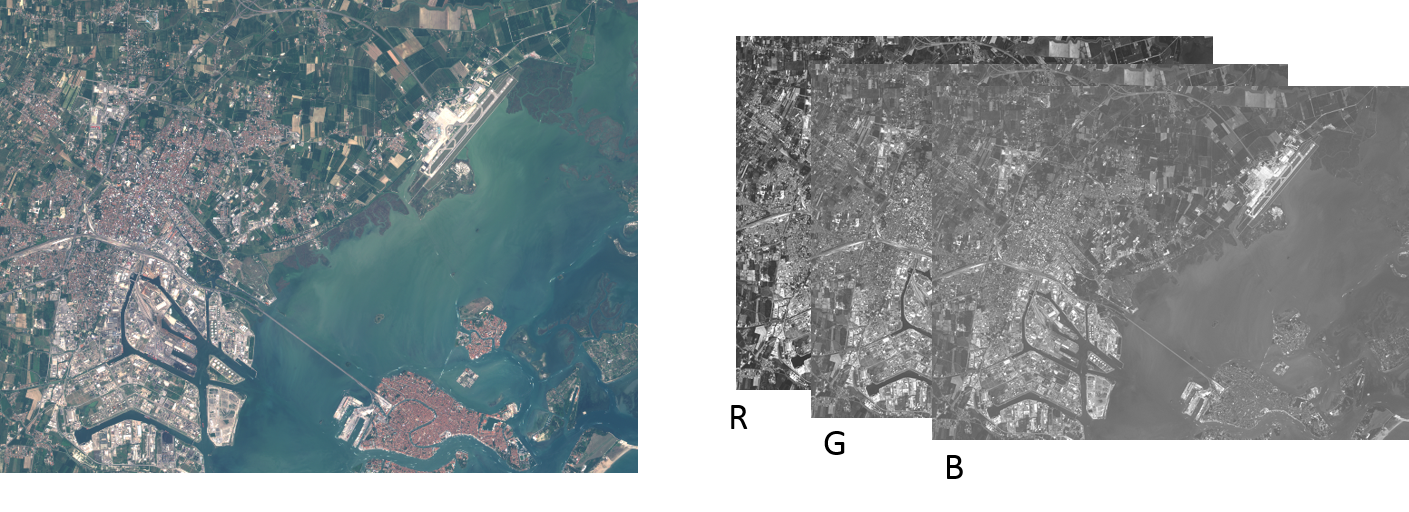
\includegraphics[width=0.75\textwidth]{veniseRGB}
  \caption{Image RGB du Nord de l'Italie (près de Venise)}
  \label{fig:veniseRGB}
\end{figure}

Une image multispectrale, quant à elle, est formée de nombreuses images prises à des longueurs d'ondes variées. On dit qu'elle est composée de plusieurs "bandes spectrales". Elle contient donc plus d'informations, et selon les longueurs d'ondes d'acquisition peut avoir, en plus du visible (400 à 800nm), des informations dans l'ultraviolet ou l'infrarouge.

\begin{figure}[H]
  \centering
    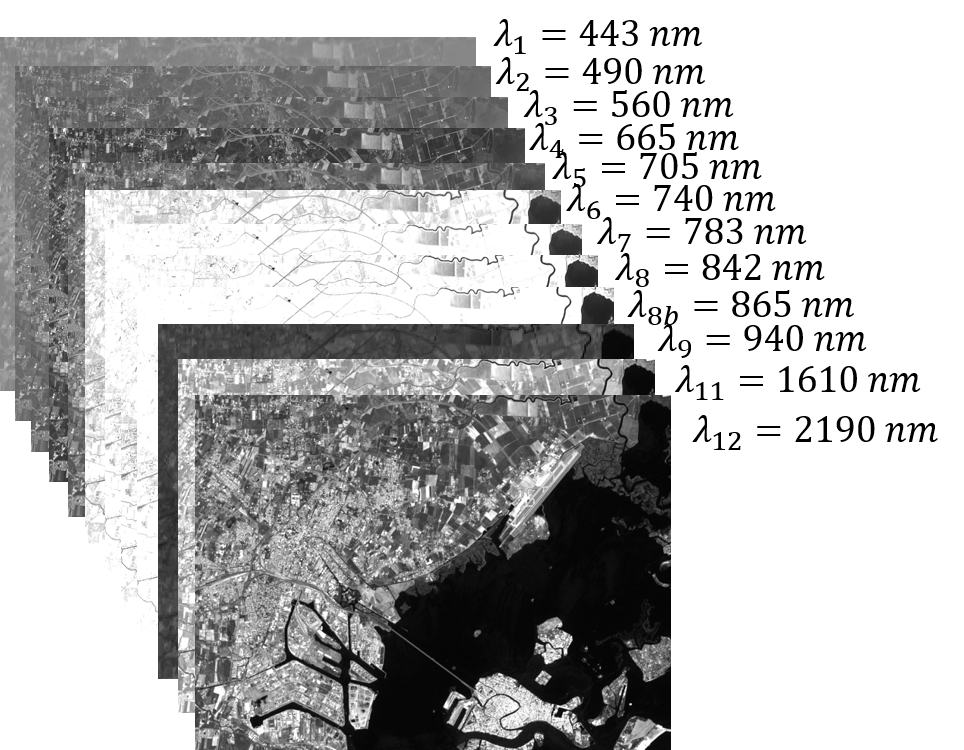
\includegraphics[width=0.5\textwidth]{multispectrale.png}
  \caption{Image multispectrale du Nord de l'Italie (près de Venise). Cette image comprend des informations dans l'infrarouge.}
  \label{fig:veniseMulti}
\end{figure}

\paragraph{MODIS vs Sentinel 2}
\paragraph{}
Parmi les satellites utilisant cette technologie on trouve les satellites Aqua et Terra MODIS (Moderate-Resolution Imaging SpectroRadiometer). Ces deux satellites, lancés par la NASA en 1999 et 2002, imagent l'intégralité de la surface de la Terre tous les deux jours. Les données sont ensuite traitées et mises à disposition du public gratuitement, ce qui en a fait une des principales sources d'images satellites multispectrales. Ces satellites sont capables de mesurer 36 bandes fréquentielles avec trois résolutions différentes: 250m, 500m et 1000m par pixel. L'objectif de cette mission est de "jouer un rôle vital dans le développement de modèles globaux, validés et interactifs de systèmes terrestres capables de prévoir des changements globaux avec suffisamment de précision pour aider les décideurs politiques à prendre des décisions avisées concernant la protection de notre environnement."\cite{nasa}

La faible résolution des données MODIS ne permet en revanche pas de discerner des détails comme des cours d'eau ou des habitations : des données plus précises sont donc nécessaires pour obtenir de meilleures classifications. 

Dans le cadre du projet \textit{Copernicus} d'observation de la Terre, l'agence spatiale européenne (ESA) développe en ce moment les missions Sentinel. Chacune de ces missions consiste en une paire de satellites en orbite autour de notre planète, récoltant des données sur la surface et l'atmosphère. Ainsi, les satellites Sentinel 2 (Sentinel 2-A lancé le 23 juin 2015 et 2-B dont le lancement est prévu pour la seconde moitié de 2016)\cite{sent2} récoltent des données multispectrales sur 13 bandes de fréquence : 4 bandes avec une résolution de 10m/pixel, 6 bandes à 20m/pixel et 3 à 60m/pixel.

\begin{figure}[H]
  \centering
    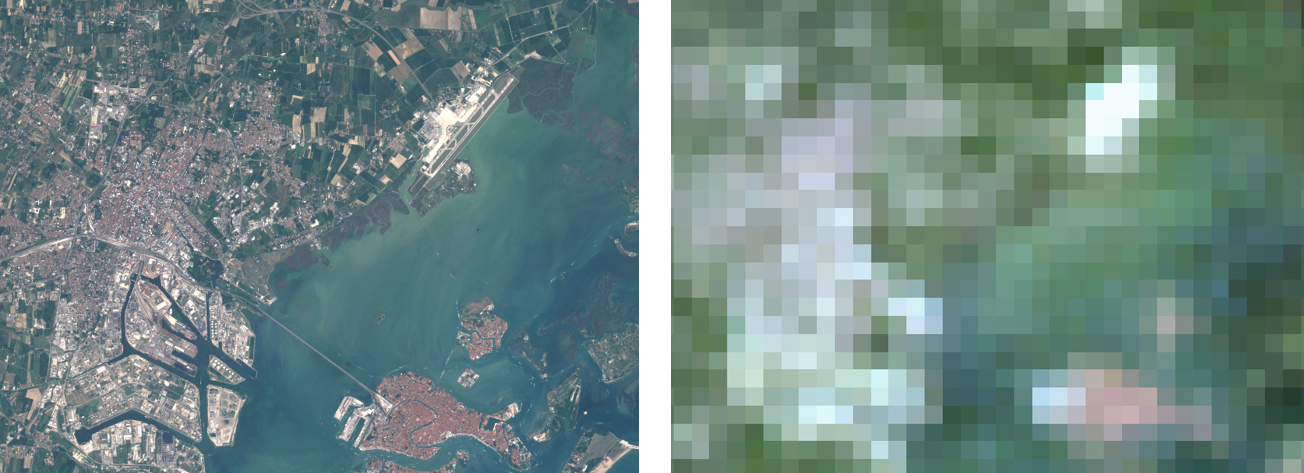
\includegraphics[width=0.75\textwidth]{SentinelVsModis.png}
  \caption{Comparaison d'une image Sentinel 2 (à g.) avec une image MODIS (à d.). Conversion des images en RGB pour faciliter la comparaison}
  \label{fig:SentinelVsModis}
\end{figure}

Les résolutions des images satellites Sentinel 2 sont de résolution grandement meilleures que celles acquises par satellites MODIS. Leur mise à disposition du public étant elle aussi gratuite, on comprend leur intérêt. 
Néanmoins, la mission de l'ESA est récente : peu de données sont actuellement disponibles. La couverture temporelle, c'est-à-dire la fréquence à laquelle le satellite passe au-dessus d'une même zone, est également assez faible. Un seul des deux satellites ayant été lancé, le renouvellement des données se fait de manière hebdomadaire, alors que les satellites MODIS renouvellent les données deux fois par jour. 

\subsection{Classification et Machine Learning}

Pour exploiter ces données, il est nécessaire de les classifier. On cherche en effet à distinguer les différentes caractéristiques des sols observés. Les données multispectrales à traiter représentant une quantité très importante, leur classification se fait à travers des algorithmes de "Machine Learning", défini en ces termes : 

\textit{L'apprentissage automatique (Machine Learning en anglais), champ d'étude de l'intelligence artificielle, concerne la conception, l'analyse, le développement et l'implémentation de méthodes permettant à une machine (au sens large) d'évoluer par un processus systématique, et ainsi de remplir des tâches difficiles ou impossibles à remplir par des moyens algorithmiques plus classiques.\footnote{\href{https://fr.wikipedia.org/wiki/Apprentissage_automatique}{Apprentissage automatique}}}

\paragraph{}
Le machine learning se sépare en trois type d'apprentissage :
\begin{itemize}
  \item[>] L'apprentissage non-supervisé, qui consiste à donner à notre algorithme uniquement les données à classifier et à le laisser établir les différentes classes à partir des ensembles qui se séparent le mieux.
  \item[>] La régression, qui cherche à définir les données à l'aide d'une loi mathématique.
  \item[>] L'apprentissage supervisé, pour lequel il faut définir, en plus des données à traiter, des ensembles de vecteurs représentatifs de chacune des classes et déjà classés. Les vecteurs classés manuellement vont servir d'entraînement pour l'apprentissage et donc pour trouver les frontières qui séparent le mieux nos différentes classes.
\end{itemize}

\paragraph{}
Dans le cas de la surveillance d'occupation des sols, on utilise souvent des méthodes supervisées, car il est relativement aisé de reconnaître à l'œil les différents types de zones au sol (eau, champs, villes, ...). Là encore, il existe plusieurs familles d'algorithmes d'apprentissage supervisé, on différenciera dans un premier temps les algorithmes linéaires et non-linéaires. Dans la famille des algorithmes non-linéaires, on trouve des algorithmes intrinsèquement multi-classes (tel que l'algorithme dit des k-plus proches voisins que nous détaillerons plus tard), et les algorithmes binaires.
%\label{DiagAlg}
\begin{center}
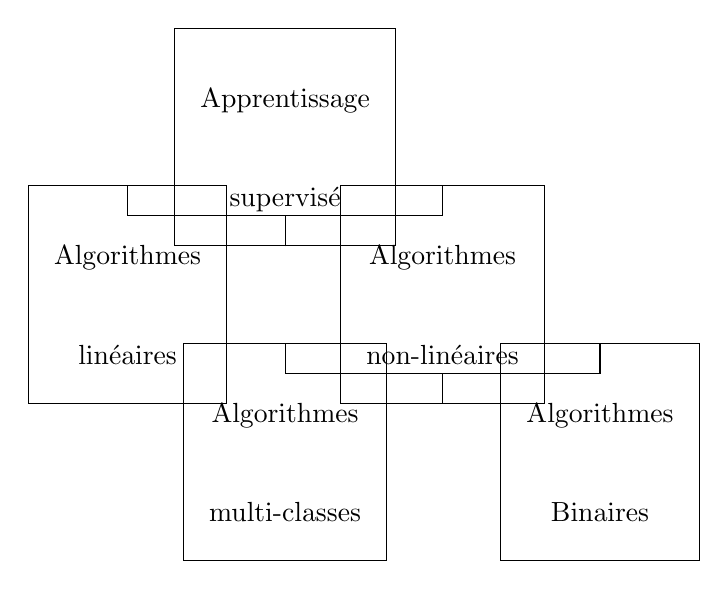
\begin{tikzpicture}
\begin{scope}
\node (AS) at (0,4.9) [rectangle,draw] {\begin{tabular}{c}Apprentissage\\ supervisé\end{tabular} };
\node (ASL) at (-2,2.9) [rectangle,draw] {\begin{tabular}{c}Algorithmes\\ linéaires\end{tabular} };
\node (ASNL) at (2,2.9) [rectangle,draw] {\begin{tabular}{c}Algorithmes\\ non-linéaires\end{tabular} };
\node (ASIM) at (0,0.9) [rectangle,draw] {\begin{tabular}{c}Algorithmes\\ multi-classes\end{tabular} };
\node (ASNM) at (4,0.9) [rectangle,draw] {\begin{tabular}{c}Algorithmes\\Binaires\end{tabular} };
\draw (AS) -- (0,3.9);
\draw (0,3.9) -| (ASNL);
\draw (0,3.9) -| (ASL);
\draw (ASNL) -- (2,1.9);
\draw (2,1.9) -| (ASIM);
\draw (2,1.9) -| (ASNM);
\end{scope}
\end{tikzpicture}
\captionof{figure}{Diagramme des différents algorithme de classification.}
\end{center}
%pas sûr que le diagramme soit utile finalement...
\paragraph{}
Pour les algorithmes intrinsèquement multi-classes, il suffit de stocker les vecteurs d'entraînement et d'appliquer directement la classification à l'ensemble des données, il n'y a donc pas d'entraînement à proprement parler.
\paragraph{}
Les algorithmes binaires, quant à eux, demandent un peu plus de travail. Dès que l'on veut traiter plus de deux classes, il faut faire plusieurs entraînements, en se ramenant chaque fois à un problème binaire. Là encore, il y a deux approches possibles en fonction des algorithmes :
 \begin{itemize}
   \item[>] La première approche s'appelle "un contre tous", elle consiste ,comme son nom l'indique, à prendre chaque classe et à l'opposer à l'ensemble des autres classes. On obtient alors n problèmes binaires et pour un élément à classifier, en cas d'ambiguïté, la classe qui obtient le plus de "votes" favorables est choisie.
   \item[>] La seconde méthode est le "un contre un", toutes les classes sont "opposées" successivement, deux à deux, et de la même façon c'est la classe qui obtient le plus de "votes" favorables qui est choisie. La principale différence réside dans le fait qu'il y ait dans ce cas ${n \choose 2}=\frac{n(n-1)}{2}$ entraînements à réaliser.
 \end{itemize}

\paragraph{L'évaluation}
\paragraph{}
Pour évaluer la qualité des résultats donnés par ces algorithmes, on procède à une phase d'entraînement suivie d'une phase de test. 
On utilise pour cela un ensemble dont on connaît les classes. On divise cet ensemble en deux sous-ensembles. 
\begin{itemize}
  \item[>]Le premier sous-ensemble contient les caractéristiques des points ainsi que leurs classes respectives. Il sert à entraîner l'algorithme. Celui-ci va ainsi apprendre quelles sont les caractéristiques de chaque classe. 
  \item[>]Le deuxième sous-ensemble contient uniquement les caractéristiques des points. Ce sous-ensemble sera classé par l'algorithme.
\end{itemize} 

On compare ensuite les classes inférées par l'algorithme aux classes attendues. On quantifie la qualité des résultats à l'aide d'un outil mathématique appelé matrice de confusion. 

\begin{figure}[H]
  \centering
    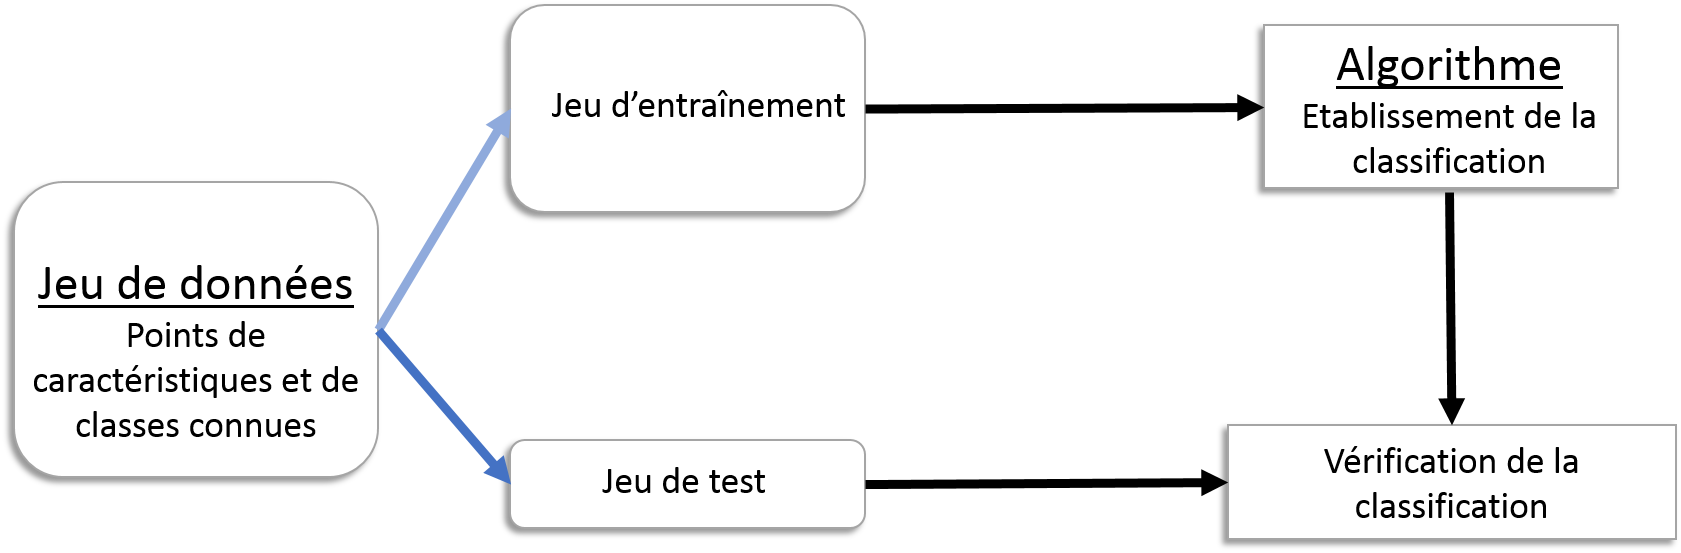
\includegraphics[width=0.75\textwidth]{mlProcess.png}
  \caption{Machine Learning}
  \label{fig:ml}
\end{figure}

\subparagraph{La matrice de confusion}
\paragraph{}
La matrice de confusion est le principal outil de mesure de la qualité d'une classification. Elle compare en effet la classification prédite par l'algorithme (en lignes) à la classification réelle (en colonnes). \ref{ConfMat}
La diagonale représente le nombre d'éléments bien classés. \newline
Plusieurs critères sont issus de cette matrice, sous forme de pourcentage. Deux critères sont donnés par classe : la \textit{précision} (precision) et le \textit{rappel} (recall). La précision est le rapport entre la quantité d'éléments bien classés et le nombre d'éléments réels de cette classe. Le rappel est le rapport entre la quantité d'éléments bien classés et le nombre d'éléments prédits par l'algorithme dans cette classe.\newline
Un autre critère est donné de manière global : l'\textcolor{red}{exactitude}(accuracy), qui est la trace de la matrice sur le nombre total d'éléments. Autrement dit, l'exactitude est le pourcentage de données bien classées. Ce résultat donne la fidélité de la classification par rapport à l'image initiale : \textbf{c'est principalement ce critère qu'on retiendra}.

\begin{figure*}
\caption{Matrice de confusion pour un exemple à trois classes.}
\label{ConfMat}
\begin{center}
\renewcommand{\arraystretch}{3}
\begin{tabular}{|c|c|c|c|c|c|}
\hline
 \multicolumn{2}{|c|}{\multirow{2}{*}{}} & \multicolumn{3}{|c}{Classes Prédites} &  \\
 \cline{3-6}
  \multicolumn{2}{|c|}{} & Classe 1 & Classe 2 & Classe 3 & Précision\\
  \hline
 \multirow{3}{*}{\begin{turn}{90} Classes Théoriques\end{turn}} & Classe 1 & $N_{11}$ & $N_{12}$ & $N_{13}$ & $\frac{N_{11}}{N_{11} + N_{12} + N_{13} }$\\
 \cline{2-6}
  & Classe 2 & $N_{21}$ & $N_{22}$ & $N_{23}$ & $\frac{N_{22}}{N_{21} + N_{22} + N_{23} }$\\
  \cline{2-6}
  & Classe 3 & $N_{31}$ & $N_{32}$ & $N_{33}$ & $\frac{N_{33}}{N_{31} + N_{32} + N_{33} }$\\
  \cline{2-6}
  & Recall  & $\frac{N_{11}}{N_{11} + N_{21} + N_{31} }$ & $\frac{N_{22}}{N_{12} + N_{22} + N_{32} }$ & $\frac{N_{33}}{N_{13} + N_{23} + N_{33} }$ & $\frac{N_{11} + N_{22} + N_{33}}{Nb echantillons}$\footnote {ce résultat donne la fidélité de la classification par rapport à l'image initiale} \\
\hline
\end{tabular}
\end{center}
\end{figure*}



\subsection{Motivation du projet et cahier des charges}

Les données Sentinel 2 étant très récentes, nous faisons partie des premiers à les analyser et aucun article à leur sujet n'a encore été publié. Leur analyse et leur classification relève donc de la recherche. 
Bien que ce projet s'étende sur une durée assez courte (6 semaines), les objectifs fixés étaient :
\begin{itemize}
  \item[>] Définir les principaux intérêts des images multispectrales Sentinel 2.
  \item[>] Établir une classification de la surface terrestre (suivi d'occupation des sols) en trois classes ("Eau", "Urbain","Champ") à partir d'une image de la base de données Sentinel 2.
  \item[>] Tester les algorithmes de Machine Learning les plus répandus.
\end{itemize}

  Dans un but de répétabilité, nous avons testé et optimisé toutes nos méthodes de machine learning sur une unique image hyperspectrale (dont une vue en RGB est donnée en figure \ref{fig:veniseRGB}).
 
